% Created by tikzDevice version 0.12.6 on 2024-02-06 12:53:47
% !TEX encoding = UTF-8 Unicode
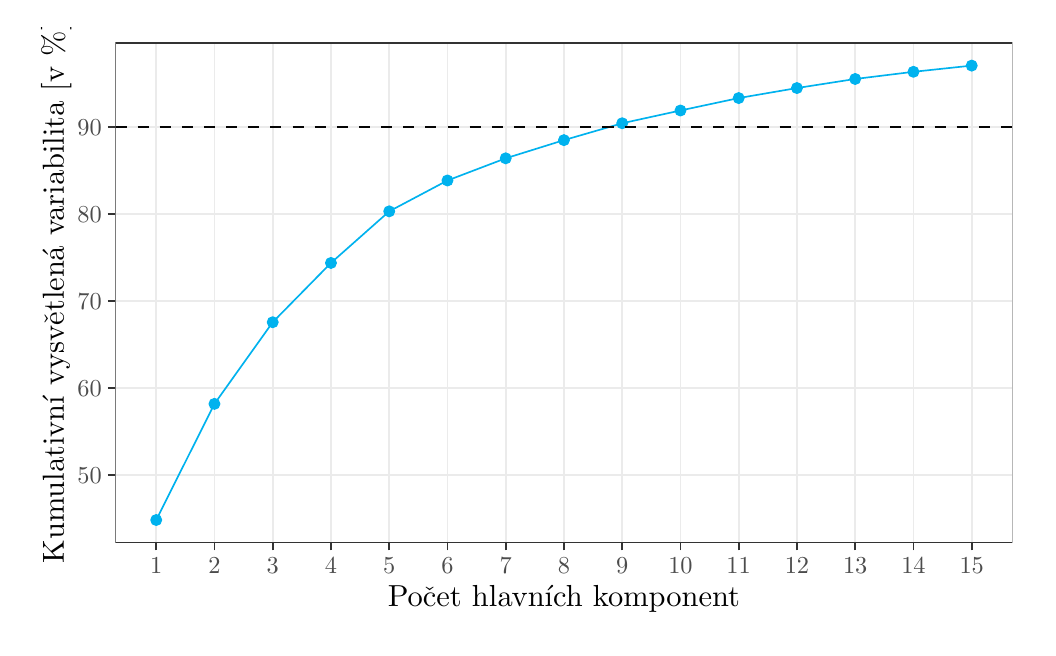
\begin{tikzpicture}[x=1pt,y=1pt]
\definecolor{fillColor}{RGB}{255,255,255}
\path[use as bounding box,fill=fillColor] (0,0) rectangle (361.35,216.81);
\begin{scope}
\path[clip] (  0.00,  0.00) rectangle (361.35,216.81);
\definecolor{drawColor}{RGB}{255,255,255}

\path[draw=drawColor,line width= 0.6pt,line join=round,line cap=round,fill=fillColor] (  0.00,  0.00) rectangle (361.35,216.81);
\end{scope}
\begin{scope}
\path[clip] ( 31.71, 30.69) rectangle (355.85,211.31);
\definecolor{fillColor}{RGB}{255,255,255}

\path[fill=fillColor] ( 31.71, 30.69) rectangle (355.85,211.31);
\definecolor{drawColor}{gray}{0.92}

\path[draw=drawColor,line width= 0.6pt,line join=round] ( 31.71, 55.25) --
	(355.85, 55.25);

\path[draw=drawColor,line width= 0.6pt,line join=round] ( 31.71, 86.64) --
	(355.85, 86.64);

\path[draw=drawColor,line width= 0.6pt,line join=round] ( 31.71,118.03) --
	(355.85,118.03);

\path[draw=drawColor,line width= 0.6pt,line join=round] ( 31.71,149.42) --
	(355.85,149.42);

\path[draw=drawColor,line width= 0.6pt,line join=round] ( 31.71,180.81) --
	(355.85,180.81);

\path[draw=drawColor,line width= 0.6pt,line join=round] ( 46.45, 30.69) --
	( 46.45,211.31);

\path[draw=drawColor,line width= 0.6pt,line join=round] ( 67.49, 30.69) --
	( 67.49,211.31);

\path[draw=drawColor,line width= 0.6pt,line join=round] ( 88.54, 30.69) --
	( 88.54,211.31);

\path[draw=drawColor,line width= 0.6pt,line join=round] (109.59, 30.69) --
	(109.59,211.31);

\path[draw=drawColor,line width= 0.6pt,line join=round] (130.64, 30.69) --
	(130.64,211.31);

\path[draw=drawColor,line width= 0.6pt,line join=round] (151.69, 30.69) --
	(151.69,211.31);

\path[draw=drawColor,line width= 0.6pt,line join=round] (172.73, 30.69) --
	(172.73,211.31);

\path[draw=drawColor,line width= 0.6pt,line join=round] (193.78, 30.69) --
	(193.78,211.31);

\path[draw=drawColor,line width= 0.6pt,line join=round] (214.83, 30.69) --
	(214.83,211.31);

\path[draw=drawColor,line width= 0.6pt,line join=round] (235.88, 30.69) --
	(235.88,211.31);

\path[draw=drawColor,line width= 0.6pt,line join=round] (256.92, 30.69) --
	(256.92,211.31);

\path[draw=drawColor,line width= 0.6pt,line join=round] (277.97, 30.69) --
	(277.97,211.31);

\path[draw=drawColor,line width= 0.6pt,line join=round] (299.02, 30.69) --
	(299.02,211.31);

\path[draw=drawColor,line width= 0.6pt,line join=round] (320.07, 30.69) --
	(320.07,211.31);

\path[draw=drawColor,line width= 0.6pt,line join=round] (341.12, 30.69) --
	(341.12,211.31);
\definecolor{drawColor}{RGB}{0,178,238}
\definecolor{fillColor}{RGB}{0,178,238}

\path[draw=drawColor,line width= 0.4pt,line join=round,line cap=round,fill=fillColor] ( 46.45, 38.90) circle (  1.96);

\path[draw=drawColor,line width= 0.4pt,line join=round,line cap=round,fill=fillColor] ( 67.49, 80.87) circle (  1.96);

\path[draw=drawColor,line width= 0.4pt,line join=round,line cap=round,fill=fillColor] ( 88.54,110.37) circle (  1.96);

\path[draw=drawColor,line width= 0.4pt,line join=round,line cap=round,fill=fillColor] (109.59,131.79) circle (  1.96);

\path[draw=drawColor,line width= 0.4pt,line join=round,line cap=round,fill=fillColor] (130.64,150.44) circle (  1.96);

\path[draw=drawColor,line width= 0.4pt,line join=round,line cap=round,fill=fillColor] (151.69,161.59) circle (  1.96);

\path[draw=drawColor,line width= 0.4pt,line join=round,line cap=round,fill=fillColor] (172.73,169.60) circle (  1.96);

\path[draw=drawColor,line width= 0.4pt,line join=round,line cap=round,fill=fillColor] (193.78,176.17) circle (  1.96);

\path[draw=drawColor,line width= 0.4pt,line join=round,line cap=round,fill=fillColor] (214.83,182.27) circle (  1.96);

\path[draw=drawColor,line width= 0.4pt,line join=round,line cap=round,fill=fillColor] (235.88,186.88) circle (  1.96);

\path[draw=drawColor,line width= 0.4pt,line join=round,line cap=round,fill=fillColor] (256.92,191.37) circle (  1.96);

\path[draw=drawColor,line width= 0.4pt,line join=round,line cap=round,fill=fillColor] (277.97,194.99) circle (  1.96);

\path[draw=drawColor,line width= 0.4pt,line join=round,line cap=round,fill=fillColor] (299.02,198.27) circle (  1.96);

\path[draw=drawColor,line width= 0.4pt,line join=round,line cap=round,fill=fillColor] (320.07,200.86) circle (  1.96);

\path[draw=drawColor,line width= 0.4pt,line join=round,line cap=round,fill=fillColor] (341.12,203.10) circle (  1.96);

\path[draw=drawColor,line width= 0.6pt,line join=round] ( 46.45, 38.90) --
	( 67.49, 80.87) --
	( 88.54,110.37) --
	(109.59,131.79) --
	(130.64,150.44) --
	(151.69,161.59) --
	(172.73,169.60) --
	(193.78,176.17) --
	(214.83,182.27) --
	(235.88,186.88) --
	(256.92,191.37) --
	(277.97,194.99) --
	(299.02,198.27) --
	(320.07,200.86) --
	(341.12,203.10);
\definecolor{drawColor}{gray}{0.02}

\path[draw=drawColor,line width= 0.6pt,dash pattern=on 4pt off 4pt ,line join=round] ( 31.71,180.81) -- (355.85,180.81);
\definecolor{drawColor}{gray}{0.20}

\path[draw=drawColor,line width= 0.6pt,line join=round,line cap=round] ( 31.71, 30.69) rectangle (355.85,211.31);
\end{scope}
\begin{scope}
\path[clip] (  0.00,  0.00) rectangle (361.35,216.81);
\definecolor{drawColor}{gray}{0.30}

\node[text=drawColor,anchor=base east,inner sep=0pt, outer sep=0pt, scale=  0.88] at ( 26.76, 52.22) {50};

\node[text=drawColor,anchor=base east,inner sep=0pt, outer sep=0pt, scale=  0.88] at ( 26.76, 83.61) {60};

\node[text=drawColor,anchor=base east,inner sep=0pt, outer sep=0pt, scale=  0.88] at ( 26.76,115.00) {70};

\node[text=drawColor,anchor=base east,inner sep=0pt, outer sep=0pt, scale=  0.88] at ( 26.76,146.39) {80};

\node[text=drawColor,anchor=base east,inner sep=0pt, outer sep=0pt, scale=  0.88] at ( 26.76,177.77) {90};
\end{scope}
\begin{scope}
\path[clip] (  0.00,  0.00) rectangle (361.35,216.81);
\definecolor{drawColor}{gray}{0.20}

\path[draw=drawColor,line width= 0.6pt,line join=round] ( 28.96, 55.25) --
	( 31.71, 55.25);

\path[draw=drawColor,line width= 0.6pt,line join=round] ( 28.96, 86.64) --
	( 31.71, 86.64);

\path[draw=drawColor,line width= 0.6pt,line join=round] ( 28.96,118.03) --
	( 31.71,118.03);

\path[draw=drawColor,line width= 0.6pt,line join=round] ( 28.96,149.42) --
	( 31.71,149.42);

\path[draw=drawColor,line width= 0.6pt,line join=round] ( 28.96,180.81) --
	( 31.71,180.81);
\end{scope}
\begin{scope}
\path[clip] (  0.00,  0.00) rectangle (361.35,216.81);
\definecolor{drawColor}{gray}{0.20}

\path[draw=drawColor,line width= 0.6pt,line join=round] ( 46.45, 27.94) --
	( 46.45, 30.69);

\path[draw=drawColor,line width= 0.6pt,line join=round] ( 67.49, 27.94) --
	( 67.49, 30.69);

\path[draw=drawColor,line width= 0.6pt,line join=round] ( 88.54, 27.94) --
	( 88.54, 30.69);

\path[draw=drawColor,line width= 0.6pt,line join=round] (109.59, 27.94) --
	(109.59, 30.69);

\path[draw=drawColor,line width= 0.6pt,line join=round] (130.64, 27.94) --
	(130.64, 30.69);

\path[draw=drawColor,line width= 0.6pt,line join=round] (151.69, 27.94) --
	(151.69, 30.69);

\path[draw=drawColor,line width= 0.6pt,line join=round] (172.73, 27.94) --
	(172.73, 30.69);

\path[draw=drawColor,line width= 0.6pt,line join=round] (193.78, 27.94) --
	(193.78, 30.69);

\path[draw=drawColor,line width= 0.6pt,line join=round] (214.83, 27.94) --
	(214.83, 30.69);

\path[draw=drawColor,line width= 0.6pt,line join=round] (235.88, 27.94) --
	(235.88, 30.69);

\path[draw=drawColor,line width= 0.6pt,line join=round] (256.92, 27.94) --
	(256.92, 30.69);

\path[draw=drawColor,line width= 0.6pt,line join=round] (277.97, 27.94) --
	(277.97, 30.69);

\path[draw=drawColor,line width= 0.6pt,line join=round] (299.02, 27.94) --
	(299.02, 30.69);

\path[draw=drawColor,line width= 0.6pt,line join=round] (320.07, 27.94) --
	(320.07, 30.69);

\path[draw=drawColor,line width= 0.6pt,line join=round] (341.12, 27.94) --
	(341.12, 30.69);
\end{scope}
\begin{scope}
\path[clip] (  0.00,  0.00) rectangle (361.35,216.81);
\definecolor{drawColor}{gray}{0.30}

\node[text=drawColor,anchor=base,inner sep=0pt, outer sep=0pt, scale=  0.88] at ( 46.45, 19.68) {1};

\node[text=drawColor,anchor=base,inner sep=0pt, outer sep=0pt, scale=  0.88] at ( 67.49, 19.68) {2};

\node[text=drawColor,anchor=base,inner sep=0pt, outer sep=0pt, scale=  0.88] at ( 88.54, 19.68) {3};

\node[text=drawColor,anchor=base,inner sep=0pt, outer sep=0pt, scale=  0.88] at (109.59, 19.68) {4};

\node[text=drawColor,anchor=base,inner sep=0pt, outer sep=0pt, scale=  0.88] at (130.64, 19.68) {5};

\node[text=drawColor,anchor=base,inner sep=0pt, outer sep=0pt, scale=  0.88] at (151.69, 19.68) {6};

\node[text=drawColor,anchor=base,inner sep=0pt, outer sep=0pt, scale=  0.88] at (172.73, 19.68) {7};

\node[text=drawColor,anchor=base,inner sep=0pt, outer sep=0pt, scale=  0.88] at (193.78, 19.68) {8};

\node[text=drawColor,anchor=base,inner sep=0pt, outer sep=0pt, scale=  0.88] at (214.83, 19.68) {9};

\node[text=drawColor,anchor=base,inner sep=0pt, outer sep=0pt, scale=  0.88] at (235.88, 19.68) {10};

\node[text=drawColor,anchor=base,inner sep=0pt, outer sep=0pt, scale=  0.88] at (256.92, 19.68) {11};

\node[text=drawColor,anchor=base,inner sep=0pt, outer sep=0pt, scale=  0.88] at (277.97, 19.68) {12};

\node[text=drawColor,anchor=base,inner sep=0pt, outer sep=0pt, scale=  0.88] at (299.02, 19.68) {13};

\node[text=drawColor,anchor=base,inner sep=0pt, outer sep=0pt, scale=  0.88] at (320.07, 19.68) {14};

\node[text=drawColor,anchor=base,inner sep=0pt, outer sep=0pt, scale=  0.88] at (341.12, 19.68) {15};
\end{scope}
\begin{scope}
\path[clip] (  0.00,  0.00) rectangle (361.35,216.81);
\definecolor{drawColor}{RGB}{0,0,0}

\node[text=drawColor,anchor=base,inner sep=0pt, outer sep=0pt, scale=  1.10] at (193.78,  7.64) {Počet hlavních komponent};
\end{scope}
\begin{scope}
\path[clip] (  0.00,  0.00) rectangle (361.35,216.81);
\definecolor{drawColor}{RGB}{0,0,0}

\node[text=drawColor,rotate= 90.00,anchor=base,inner sep=0pt, outer sep=0pt, scale=  1.10] at ( 13.08,121.00) {Kumulativní vysvětlená variabilita [v \%]};
\end{scope}
\end{tikzpicture}
